\section{Adapting UQ Methods to FC}
\label{sec:discussion}


The results from \Cref{sec:benchmark} suggest that the more involved entropy-based multi-sample UQ methods we evaluate underperform compared to simple single-sample methods. 
This contrasts with observations in natural language generation tasks. 
In the following, we investigate two hypotheses around this observation. 
In this section, we investigate whether the performance of existing UQ methods in the FC setting can be improved by adapting them to the particular structure of FC outputs.









\subsection{Adapting Multi-Sample UQ Methods} 
\label{sec:SE_AST}

% \begin{wraptable}{r}{0.6\textwidth}
% 






\centering
\resizebox{0.55\textwidth}{!}{\begin{tabular}{l|cc|cc}

\toprule
\textbf{Task} & \textbf{SE}$_{EXM}$ & \textbf{SE}$_{AST}$ & \textbf{DSE}$_{EXM}$ & \textbf{DSE}$_{AST}$ \\ 
\hline
\textbf{Simple} & $0.73$ \tiny{±$.049$} & \best{$0.75$} \tiny{±$.047$} & $0.73$ \tiny{±$.049$} & \best{$0.75$} \tiny{±$.047$} \\
\textbf{Multiple} & $0.73$ \tiny{±$.073$} & \best{$0.75$} \tiny{±$.067$} & $0.73$ \tiny{±$.073$} & \best{$0.74$} \tiny{±$.067$} \\
\textbf{Parallel} & $0.66$ \tiny{±$.059$} & \best{$0.69$} \tiny{±$.056$} & $0.66$ \tiny{±$.059$} & \best{$0.69$} \tiny{±$.056$} \\
\textbf{Parallel-Multiple} & $0.73$ \tiny{±$.051$} & \best{$0.74$} \tiny{±$.049$} & \best{$0.73$} \tiny{±$.051$} & \best{$0.73$} \tiny{±$.049$} \\
\textbf{Simple + Multiple} & $0.73$ \tiny{±$.041$} & \best{$0.75$} \tiny{±$.038$} & $0.73$ \tiny{±$.041$} & \best{$0.75$} \tiny{±$.038$} \\
\textbf{Simple + Parallel} & $0.71$ \tiny{±$.038$} & \best{$0.73$} \tiny{±$.036$} & $0.70$ \tiny{±$.038$} & \best{$0.73$} \tiny{±$.036$} \\
\textbf{Multiple + Parallel-Multiple} & $0.74$ \tiny{±$.041$} & \best{$0.76$} \tiny{±$.038$} & $0.73$ \tiny{±$.041$} & \best{$0.75$} \tiny{±$.038$} \\
\textbf{All Combined} & $0.72$ \tiny{±$.027$} & \best{$0.74$} \tiny{±$.026$} & $0.72$ \tiny{±$.027$} & \best{$0.74$} \tiny{±$.026$} \\
\textbf{Simple + Irrelevance} & \best{$0.76$} \tiny{±$.026$} & $0.75$ \tiny{±$.025$} & \best{$0.76$} \tiny{±$.026$} & $0.74$ \tiny{±$.025$} \\
\textbf{All Combined + Irrelevance} & \best{$0.74$} \tiny{±$.020$} & \best{$0.74$} \tiny{±$.020$} & \best{$0.74$} \tiny{±$.020$} & $0.73$ \tiny{±$.020$} \\
\bottomrule
\end{tabular}}


\caption{
Mean AUROC, $\pm$ mean standard error (mean taken over the eight LLMs) for all tasks from \Cref{sec:benchmark}.
}

% \label{tab:new_method_se}
% \end{wraptable}



In the following, we investigate whether multi-sample UQ methods can be tailored to the FC setting. Specifically, we focus on the two variants of Semantic Entropy (SE and DSE) as the highest-performing multi-sequence methods.

The original SE implementation clusters generations with an LLM-based entailment model. We report in \Cref{app:SEentail} that this does not transfer to FC outputs: entailment-based clustering is substantially worse than exact string matching, which we attribute to textual entailment being the wrong equivalence relation for structured outputs. This motivates the structural alternative we consider here.

We hypothesize that the clustering based on exact string matching (EXM) used in our experiments might be overly strict, as it does not take permutation invariance in the function arguments into account.
To circumvent this, we utilize the Abstract Syntax Trees (\textbf{AST}) to cluster FC outputs based on \citet{bfcl}. Two outputs get assigned the same cluster if their AST matches. This approach effectively treats the arguments to the function as a dictionary that is permutation-invariant.

% \begin{wraptable}{r}{0.6\textwidth}
% 






\centering
\resizebox{0.55\textwidth}{!}{\begin{tabular}{l|cc|cc}

\toprule
\textbf{Task} & \textbf{SE}$_{EXM}$ & \textbf{SE}$_{AST}$ & \textbf{DSE}$_{EXM}$ & \textbf{DSE}$_{AST}$ \\ 
\hline
\textbf{Simple} & $0.73$ \tiny{±$.049$} & \best{$0.75$} \tiny{±$.047$} & $0.73$ \tiny{±$.049$} & \best{$0.75$} \tiny{±$.047$} \\
\textbf{Multiple} & $0.73$ \tiny{±$.073$} & \best{$0.75$} \tiny{±$.067$} & $0.73$ \tiny{±$.073$} & \best{$0.74$} \tiny{±$.067$} \\
\textbf{Parallel} & $0.66$ \tiny{±$.059$} & \best{$0.69$} \tiny{±$.056$} & $0.66$ \tiny{±$.059$} & \best{$0.69$} \tiny{±$.056$} \\
\textbf{Parallel-Multiple} & $0.73$ \tiny{±$.051$} & \best{$0.74$} \tiny{±$.049$} & \best{$0.73$} \tiny{±$.051$} & \best{$0.73$} \tiny{±$.049$} \\
\textbf{Simple + Multiple} & $0.73$ \tiny{±$.041$} & \best{$0.75$} \tiny{±$.038$} & $0.73$ \tiny{±$.041$} & \best{$0.75$} \tiny{±$.038$} \\
\textbf{Simple + Parallel} & $0.71$ \tiny{±$.038$} & \best{$0.73$} \tiny{±$.036$} & $0.70$ \tiny{±$.038$} & \best{$0.73$} \tiny{±$.036$} \\
\textbf{Multiple + Parallel-Multiple} & $0.74$ \tiny{±$.041$} & \best{$0.76$} \tiny{±$.038$} & $0.73$ \tiny{±$.041$} & \best{$0.75$} \tiny{±$.038$} \\
\textbf{All Combined} & $0.72$ \tiny{±$.027$} & \best{$0.74$} \tiny{±$.026$} & $0.72$ \tiny{±$.027$} & \best{$0.74$} \tiny{±$.026$} \\
\textbf{Simple + Irrelevance} & \best{$0.76$} \tiny{±$.026$} & $0.75$ \tiny{±$.025$} & \best{$0.76$} \tiny{±$.026$} & $0.74$ \tiny{±$.025$} \\
\textbf{All Combined + Irrelevance} & \best{$0.74$} \tiny{±$.020$} & \best{$0.74$} \tiny{±$.020$} & \best{$0.74$} \tiny{±$.020$} & $0.73$ \tiny{±$.020$} \\
\bottomrule
\end{tabular}}


\caption{
Mean AUROC, $\pm$ mean standard error (mean taken over the eight LLMs) for all tasks from \Cref{sec:benchmark}.
}

% \label{tab:new_method_se}
% \end{wraptable}

\paragraph{Results}
\Cref{tab:new_method_se} suggests that AST clustering improves performance over simple EXM clustering in eight out of ten tasks. However, these gains remain insufficient to establish an advantage over single-sample methods.
We note that multi-sample methods also require proportionally higher throughput (proportional to the number of samples $J$), which is non-negligible especially in on-device scenarios.
We further ablate the choice of temperature $T$ and number of samples $J$ in \Cref{app:sensitivity}: while increasing $T$ to $1.5$ or $J$ to $30$ can close the gap to G-NLL, it does not surpass it on most tasks.
This raises the question of why multi-sample UQ methods do not perform better in comparison, despite incorporating multiple samples. To better understand this limitation, we conduct a more detailed analysis in the following.

\begin{table*}[!htbp]







\centering
\resizebox{0.55\textwidth}{!}{\begin{tabular}{l|cc|cc}

\toprule
\textbf{Task} & \textbf{SE}$_{EXM}$ & \textbf{SE}$_{AST}$ & \textbf{DSE}$_{EXM}$ & \textbf{DSE}$_{AST}$ \\ 
\hline
\textbf{Simple} & $0.73$ \tiny{±$.049$} & \best{$0.75$} \tiny{±$.047$} & $0.73$ \tiny{±$.049$} & \best{$0.75$} \tiny{±$.047$} \\
\textbf{Multiple} & $0.73$ \tiny{±$.073$} & \best{$0.75$} \tiny{±$.067$} & $0.73$ \tiny{±$.073$} & \best{$0.74$} \tiny{±$.067$} \\
\textbf{Parallel} & $0.66$ \tiny{±$.059$} & \best{$0.69$} \tiny{±$.056$} & $0.66$ \tiny{±$.059$} & \best{$0.69$} \tiny{±$.056$} \\
\textbf{Parallel-Multiple} & $0.73$ \tiny{±$.051$} & \best{$0.74$} \tiny{±$.049$} & \best{$0.73$} \tiny{±$.051$} & \best{$0.73$} \tiny{±$.049$} \\
\textbf{Simple + Multiple} & $0.73$ \tiny{±$.041$} & \best{$0.75$} \tiny{±$.038$} & $0.73$ \tiny{±$.041$} & \best{$0.75$} \tiny{±$.038$} \\
\textbf{Simple + Parallel} & $0.71$ \tiny{±$.038$} & \best{$0.73$} \tiny{±$.036$} & $0.70$ \tiny{±$.038$} & \best{$0.73$} \tiny{±$.036$} \\
\textbf{Multiple + Parallel-Multiple} & $0.74$ \tiny{±$.041$} & \best{$0.76$} \tiny{±$.038$} & $0.73$ \tiny{±$.041$} & \best{$0.75$} \tiny{±$.038$} \\
\textbf{All Combined} & $0.72$ \tiny{±$.027$} & \best{$0.74$} \tiny{±$.026$} & $0.72$ \tiny{±$.027$} & \best{$0.74$} \tiny{±$.026$} \\
\textbf{Simple + Irrelevance} & \best{$0.76$} \tiny{±$.026$} & $0.75$ \tiny{±$.025$} & \best{$0.76$} \tiny{±$.026$} & $0.74$ \tiny{±$.025$} \\
\textbf{All Combined + Irrelevance} & \best{$0.74$} \tiny{±$.020$} & \best{$0.74$} \tiny{±$.020$} & \best{$0.74$} \tiny{±$.020$} & $0.73$ \tiny{±$.020$} \\
\bottomrule
\end{tabular}}


\caption{
Mean AUROC, $\pm$ mean standard error (mean taken over the eight LLMs) for all tasks from \Cref{sec:benchmark}.
}

\label{tab:new_method_se}
\end{table*}


\subsection{Patterns of Token Probabilities in FC vs.\ Natural Language Tasks}
\label{sec:discussion_se}




To better understand why SE and DSE still do not outperform single-sample methods like G-NLL, we investigate an example of a wrong response by Qwen2.5-7B-Instruct to a request from the \emph{Parallel-Multiple} task in \Cref{fig:example_SE_failure1} 
(full description of question and available functions in \Cref{app:parallel-multiple_example}). 
Here, the LLM makes the mistake of adding an unexpected parameter at the end of the last function call (\texttt{year=1882}). 
This example illustrates two patterns that we find to hold in general:
\begin{enumerate}[leftmargin=*, topsep=0pt, itemsep=2pt, partopsep=0pt, parsep=0pt]
\item The LLM assigns high probabilities (probability $\approx 1$) to most tokens and exhibits only a minimal degree of uncertainty at a small number of tokens ($<5$), including those associated with the error.
\item Even for tokens the LLM is slightly uncertain about (probability $<1$), the second most likely token is either semantically equivalent (\texttt{=["} vs. \texttt{=['}) or is significantly less likely (\texttt{year} vs. \texttt{specific}).
\end{enumerate}


As a result, the samples for computing the multi-sample methods are all semantically identical to the greedy-decoded one, differing only in syntactically equivalent tokens \texttt{=["} vs. \texttt{=['}.
Consequently, only a single semantic cluster is formed, resulting in low SE, even though the response is incorrect.

We compare this to a wrong response the same LLM gives to a natural language question from Natural Questions (NQ) dataset \cite{kwiatkowski2019natural} in \Cref{app:nq}. 
In this setting, neither of the above two patterns holds.
In the FC setting, where available functions are provided in-context and the valid output space is restricted, the probabilities of individual tokens are higher than in natural language settings. 
Indeed, across the eight LLMs, we find that the average token probability on \emph{All Combined} is $0.97$,\footnote{This also explains the large overconfidence of AVG in \Cref{sec:calibration}, as the average accuracy on \textit{All Combined} is $<0.9$.} while for the NQ dataset it is only $0.71$. 
Similarly, the mean number of semantic clusters formed and corresponding SE estimates are significantly lower on BFCL than on NQ ($3.4$ vs. $6.4$).%

In contrast, single-sample methods like G-NLL rely directly on the sequence probability, making them sensitive to variations in the few tokens where the LLM assigns probabilities lower than 1.
However, \Cref{fig:example_SE_failure1} highlights a limitation of single-sample methods in their current form: The impact of lower probabilities for semantically unimportant tokens (the token \texttt{=["} is required by the function description) might distort their score.
Our knowledge about the structure of function calls and which tokens carry semantic weight raises the question of whether single-sample methods can be adapted to better leverage these characteristics of FC outputs.



\subsection{Adapting Single-Sample UQ Methods}
\label{sec:new_method} 


In the following, we implement a method that aims to address the limitation of single-sample methods. 
We first analyze which tokens are semantically meaningful in the FC context (as opposed to syntactically required ones) and derive a general algorithm to extract those from an FC output. 

\paragraph{Semantically Meaningful Tokens}
We define Semantically Meaningful Tokens in the FC context as those corresponding to positions where the LLM has to decide between tokens that likely lead to either correct or incorrect outputs. Using the example response in \Cref{fig:example_SE_failure1}, these are:
\begin{enumerate}[leftmargin=*, topsep=0pt, itemsep=2pt, partopsep=0pt, parsep=0pt]
    \item \textcolor{pink1}{\rule{1.2ex}{1.2ex}} Tokens deciding if functions are called or the task is refused (the first token: \texttt{[})
    \item \textcolor{yellow2}{\rule{1.2ex}{1.2ex}} Tokens deciding if the right function is called (\texttt{history}, \texttt{get}, \texttt{get})
    \item \textcolor{green3}{\rule{1.2ex}{1.2ex}} Tokens deciding if the right parameter is used 
    (
    \texttt{country}, 
    \texttt{start}, 
    \texttt{end}, 
    \texttt{event}, 
    \texttt{(s}, 
    \texttt{artist}, 
    \texttt{(s}, 
    \texttt{artist}, 
    \texttt{year}). 
    \item \textcolor{blue4}{\rule{1.2ex}{1.2ex}} Tokens deciding if the right parameter value is chosen (
    \texttt{1}, \texttt{8}, \texttt{0}, \texttt{0}, \texttt{1}, \texttt{9}, \texttt{0}, \texttt{0}, \texttt{War}, \texttt{,}, \texttt{E}, \texttt{conomy}, \texttt{The} \texttt{Thinker}, \texttt{August}, \texttt{e}, \texttt{Rod}, \texttt{in}, \texttt{The}, \texttt{Kiss}, \texttt{August}, \texttt{e}, \texttt{Rod}, \texttt{in})
    \item \textcolor{cyan5}{\rule{1.2ex}{1.2ex}} Tokens deciding if the right number of functions is called (\texttt{])}, \texttt{ ,)}, \texttt{ )]})
    \item \textcolor{purple6}{\rule{1.2ex}{1.2ex}} Tokens deciding if the right number of parameters are included in a call (\texttt{",}, \texttt{ ,}, \texttt{ ,}, \texttt{ ])}, \texttt{ ",}, \texttt{ ",})
\end{enumerate}


All remaining tokens are primarily syntactically required to form a correct function call output (such as \texttt{=}), or continuations of function names according to the available names in the context (such as \texttt{cul}, \texttt{pt}, \texttt{ure}). 
Under this definition, in the above example, the semantically meaningful tokens would include the token \texttt{year}, which has higher uncertainty and is related to the LLM's mistake. In contrast, the token \texttt{=["} would not be included, which should not have high uncertainty, since the function format requires the parameter value in the form of an array, making this token syntactically necessary.
While this logic can be argued about and other ways of defining semantically meaningful tokens could be considered, we find that even this simple heuristic already yields improvements in UQ performance. Lastly, we highlight that this approach is related to previous work that proposes to focus on relevant tokens when computing UQ scores \cite{duan2023shifting, fadeeva2024fact, bakman2024mars}. However, these methods are tailored to the context of natural language and no such approach has been proposed for the FC setting so far.



\begin{wrapfigure}[41]{r}{0.5\linewidth}
\centering
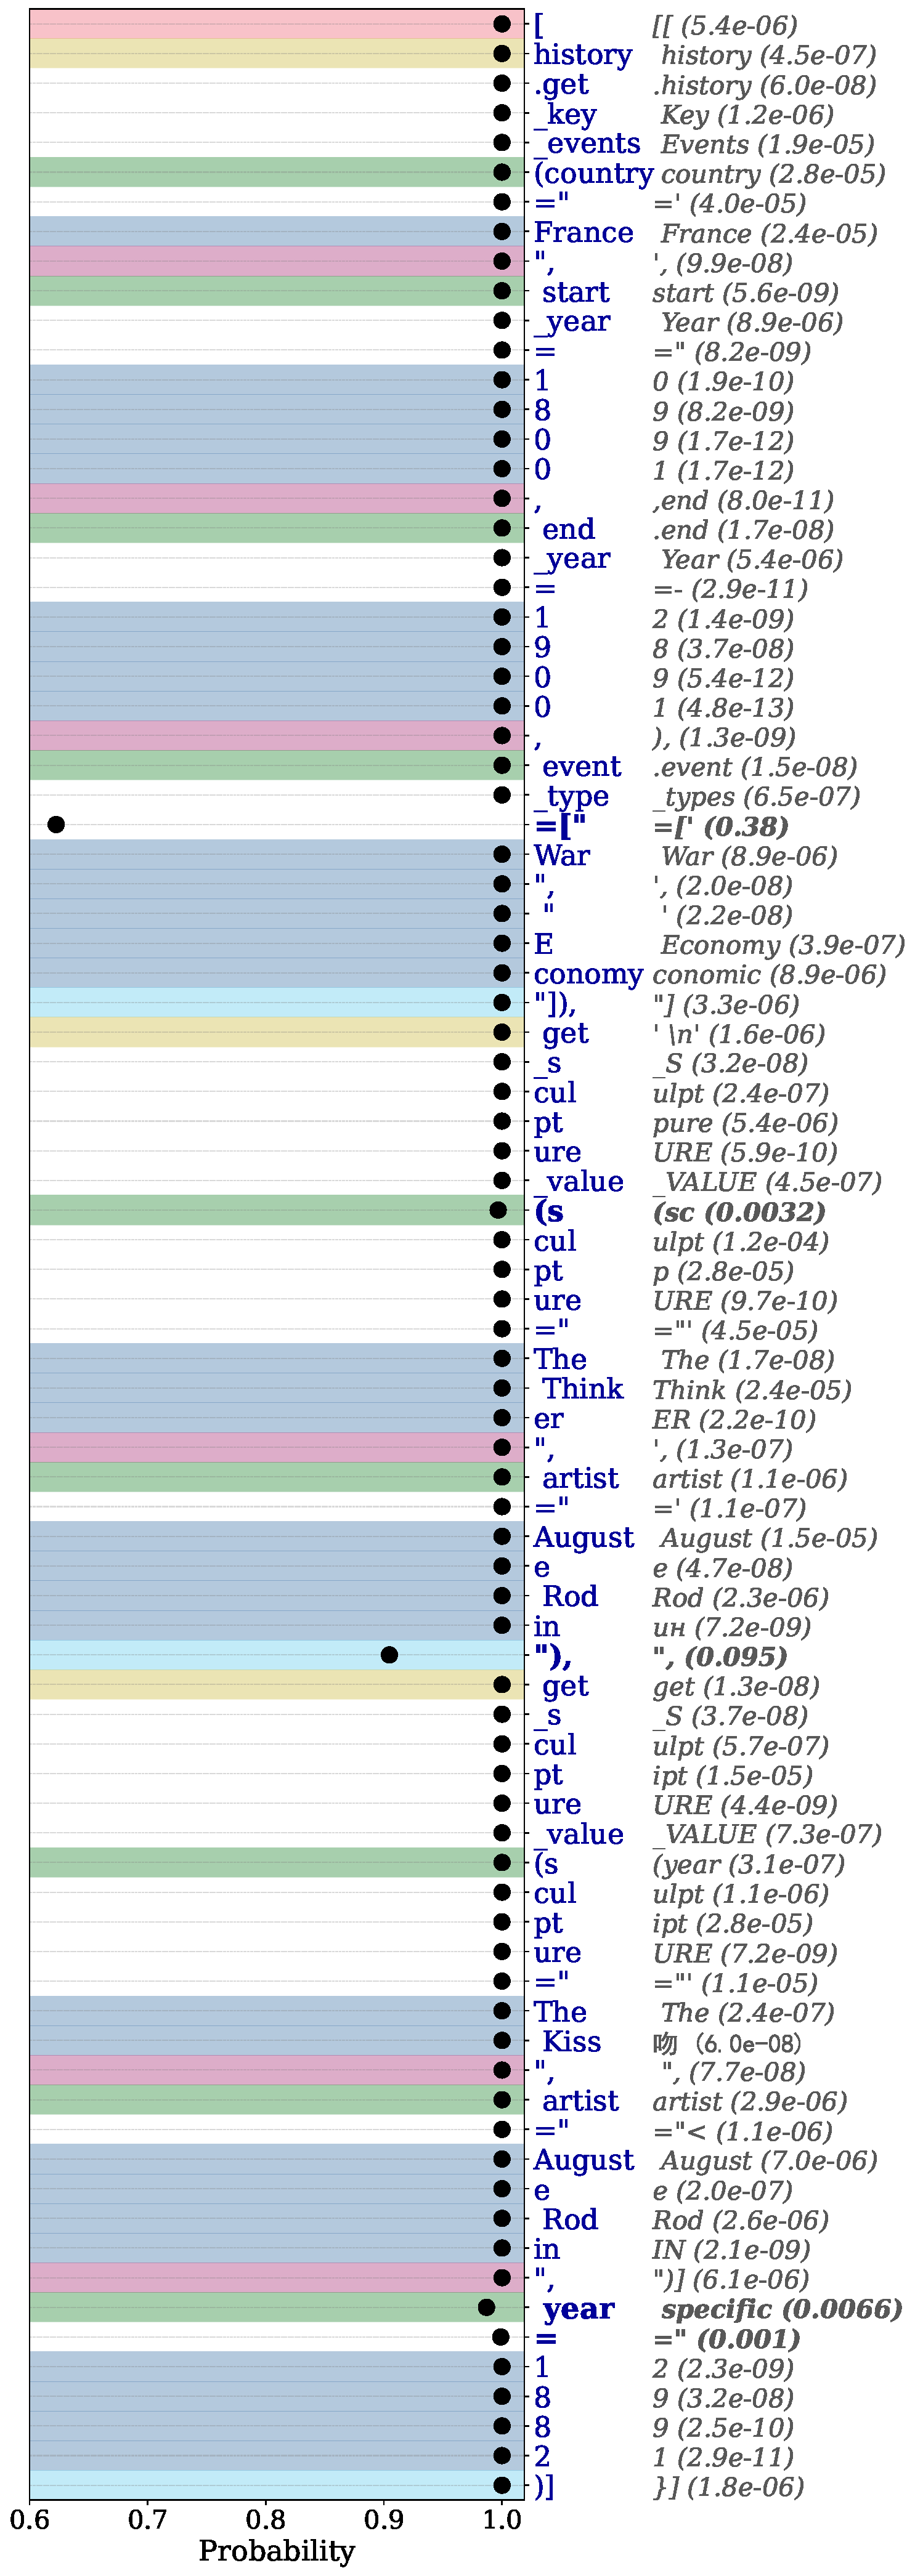
\includegraphics[width=0.6\linewidth]{figures/token_probs_auguste.pdf}
\caption{\raggedright{
Top token probabilities for an incorrect Qwen2.5-7B-Instruct response (lowest 5 in bold) in the \emph{Multiple-Parallel} task (details in \Cref{app:parallel-multiple_example}). Second-highest tokens shown in grey. Color coding explained in \Cref{sec:new_method}. The Ground truth answer does not contain the argument
\texttt{year=1882}.
}}
\label{fig:example_SE_failure1}
\end{wrapfigure}

\paragraph{Implementing SMT Extraction}
Once defined, there are many options to extract the semantically meaningful tokens from a given LLM function-call output. We opt for a simple, rule-based approach that is both computationally efficient and easy to implement. Nonetheless, it requires a separate implementation for different FC output formats, depending on the LLM's specific instruction used for finetuning. For the models evaluated, gemma and Qwen models share the same FC output format corresponding to a list of Python calls (see \Cref{fig:example_SE_failure1}), while Ministral outputs its function calls in a JSON format and thus requires a separate implementation of the token extraction function. We include the algorithms for both in \Cref{app:new_method}.
Note that this extraction operates purely on the syntactic structure of the model's own output tokens and never accesses the gold function call, so it is label-free and cannot leak ground-truth information into the UQ score.

We note that the extraction logic follows from the formal grammar of the output schema/format used for AST parsing, and only a handful of FC output schemas account for the majority of LLM FC use. To further demonstrate the ease of adapting the SMT extraction to new formats, we prompted GPT-5.2 with 10 examples each of Qwen7B and Ministral function-call outputs together with our Python-format SMT algorithm, asking it to produce the corresponding algorithm for the Ministral JSON format. The resulting function selected on average $57\%$ of Ministral-generated tokens as semantically meaningful, compared to $54\%$ by our manually written algorithm, selecting nearly identical tokens. The performance impact was minimal: on average $0.001$ AUROC difference over the 10 splits, with a maximum divergence of $0.004$ (on \emph{Simple}).


Once the semantically meaningful tokens are defined and extracted, we aggregate the corresponding log-probabilities in the same way as for the whole token sequence (MAX, G-NLL, AVG). This leads to an adaptation of single-sample methods to the FC setting we refer to as \textbf{SMT}.




\setlength{\tabcolsep}{10pt}








\begin{wraptable}{r}{0.5\textwidth}
\vspace{-40pt}
\centering
\resizebox{0.4\textwidth}{!}{\begin{tabular}{l|cc}
\toprule
\textbf{Task} & \textbf{G-NLL} & \method  \\
\hline
\textbf{Simple} & {$0.77$} \tiny{±$.045$} & \best{$0.78$} \tiny{±$.047$} \\
\textbf{Multiple} & \best{$0.76$} \tiny{±$.065$} & \best{$0.76$} \tiny{±$.065$} \\
\textbf{Parallel} & {$0.71$} \tiny{±$.058$} & \best{$0.73$} \tiny{±$.057$} \\
\textbf{Parallel-Multiple} & {$0.76$} \tiny{±$.048$} & \best{$0.78$} \tiny{±$.044$} \\
\textbf{Simple + Multiple} & {$0.77$} \tiny{±$.037$} & \best{$0.78$} \tiny{±$.038$} \\
\textbf{Simple + Parallel} & {$0.75$} \tiny{±$.036$} & \best{$0.76$} \tiny{±$.036$} \\
\textbf{Multiple + Parallel-Multiple} & {$0.77$} \tiny{±$.037$} & \best{$0.79$} \tiny{±$.035$} \\
\textbf{All Combined} & {$0.76$} \tiny{±$.025$} & \best{$0.78$} \tiny{±$.025$} \\
\textbf{Simple + Irrelevance} & {$0.81$} \tiny{±$.025$} & \best{$0.82$} \tiny{±$.025$} \\
\textbf{All Combined + Irrelevance} & {$0.78$} \tiny{±$.020$} & \best{$0.80$} \tiny{±$.019$} \\

\bottomrule
\end{tabular}}
\caption{
Mean AUROC, $\pm$ mean standard error (mean taken over the eight LLMs) for all tasks from \Cref{sec:benchmark}.%
}
\label{tab:new_method}
\end{wraptable}


\vspace{-5pt}
\paragraph{Results}



\Cref{tab:new_method} shows the performance of G-NLL$_{SMT}$ compared to G-NLL, which has emerged as the dominant method in \Cref{sec:individual_tasks}-\ref{sec:irrelevance_combinations}.
On three out of the four individual tasks, G-NLL$_{SMT}$ performs better than G-NLL. 
It also performs better on all of the combinations of tasks, including those that involve unanswerable questions. While the observed gains are only small, they are consistent.
We caution, however, that these AUROC gains are not statistically significant: a paired Wilcoxon signed-rank test across models (\Cref{app:paired_significance}) finds no systematic advantage of G-NLL$_{SMT}$ over G-NLL, with the per-task median $\Delta$AUROC small in magnitude and split in both directions.
In \Cref{app:detailed_results} we show that the same is true for MAX$_{SMT}$ and AVG$_{SMT}$.
Furthermore, SMT also improves calibration of G-NLL and MAX on almost all tasks. For example, on \textit{All Combined}, the smoothECE is dropping from $0.147$ for G-NLL to $0.091$ for G-NLL$_{SMT}$ and from $0.075$ for MAX to $0.053$ for MAX$_{SMT}$ (the impact on AVG is insignificant). The full calibration results can be found in \Cref{app:calibration}.

The differences are somewhat more consistent under the selective-prediction metrics, which measure the utility of a score under abstention rather than its ranking quality alone. In \Cref{app:selection_pred_metrics}, G-NLL$_{SMT}$ attains the best NAURC on 9 of the 10 splits and the best prediction-rejection ratio on all 10 splits at PRR$@50\%$, and it is at least as good as G-NLL on every split at both rejection rates. The margins are small, however, and we do not test them for significance, so we read this as a consistent trend in direction rather than a demonstrated improvement. A possible explanation is that AUROC summarizes the ranking over the whole score range, whereas NAURC and PRR weight the low-uncertainty region in which abstention decisions are made, so a modification that mainly affects the ordering among the most uncertain outputs would be more visible under the latter. Overall we regard SMT as a cheap modification that does not hurt and tends to help slightly---most clearly in calibration---rather than one that reliably improves UQ performance in this setting.

Overall, we thus find that the particularities of FC outputs can be leveraged when designing UQ methods for this setting, though to different degrees. AST-based clustering yields a consistent improvement over exact-match clustering for the multi-sample methods, whereas restricting single-sample scores to semantically meaningful tokens leaves discrimination essentially unchanged, improves calibration, and yields small, untested gains in the selective-prediction metrics.






\section{Conclusion}
We present the first benchmark for UQ methods in LLM Function-Calling (FC) settings. %
We show that in FC settings, simple logit-based UQ methods largely perform better than the more sophisticated entropy-based multi-sample methods we evaluate. %
We further show that the particularities of the FC setting can be utilized to improve existing UQ methods. Specifically, we adapt the semantic-entailment method of multi-sample UQ methods by using Abstract Syntax Trees. For single-sample UQ methods, we use only semantically meaningful tokens, which we define by analyzing FC outputs, when calculating their UQ scores. AST-based clustering consistently improves over exact-match clustering, while the semantically-meaningful-token variant leaves discrimination essentially unchanged and instead improves calibration, with smaller gains in the selective-prediction metrics. %




\section{Limitations}

We see three main limitations to this work. First, it would be interesting to compare how our analysis holds for the frontier models that top the BFCL benchmark. However, these tend to not disclose token probabilities through their API, and for those which are open-source, they are computationally infeasible to run on our hardware. Also, we believe that our findings for smaller and medium-sized models are still very relevant, especially in the context of on-device function calling, which would need to rely on such smaller models.
Second, it would be interesting to conduct this analysis also for more challenging function-calling settings, such as in multi-turn or agent settings. We leave this analysis for future research.

Third, the multi-sample baselines we evaluate are entropy-based: predictive entropy and the SE/DSE family. Other families of sampling-based estimators that we do not evaluate here include similarity-graph methods such as DegMat, Eccentricity and EigenValue \citep{lin2024gener}, hybrid scores that combine sample similarity with sequence likelihood such as CoCoA \citep{vashurin2025uncer}, and representation-based estimators computed from hidden states such as EigenScore \citep{chen2024insid}. Since the output-space signal is compressed in the FC setting (\Cref{sec:discussion_se}), these estimators may behave differently from the entropy-based ones, and evaluating them---which can reuse the same sample budget---is an important direction for future work. Our conclusions should therefore be read as applying to the entropy-based multi-sample methods we evaluate rather than to sampling-based UQ in general.

